\documentclass[12pt,letter]{article}
\usepackage{graphicx}
\usepackage[left=1in,right=1in]{geometry}
\usepackage{hyperref}
\hypersetup{
    colorlinks=true,
    linkcolor=blue,
    filecolor=magenta,      
    urlcolor=cyan,
    pdftitle={Overleaf Example},
    pdfpagemode=FullScreen,
    }
\begin{document}

\title{ML classification as a means of peak deconvolution}
\author{Shadrach Kwakye-Nimo}
\maketitle



\begin{figure}[!htb]
	\begin{center}
	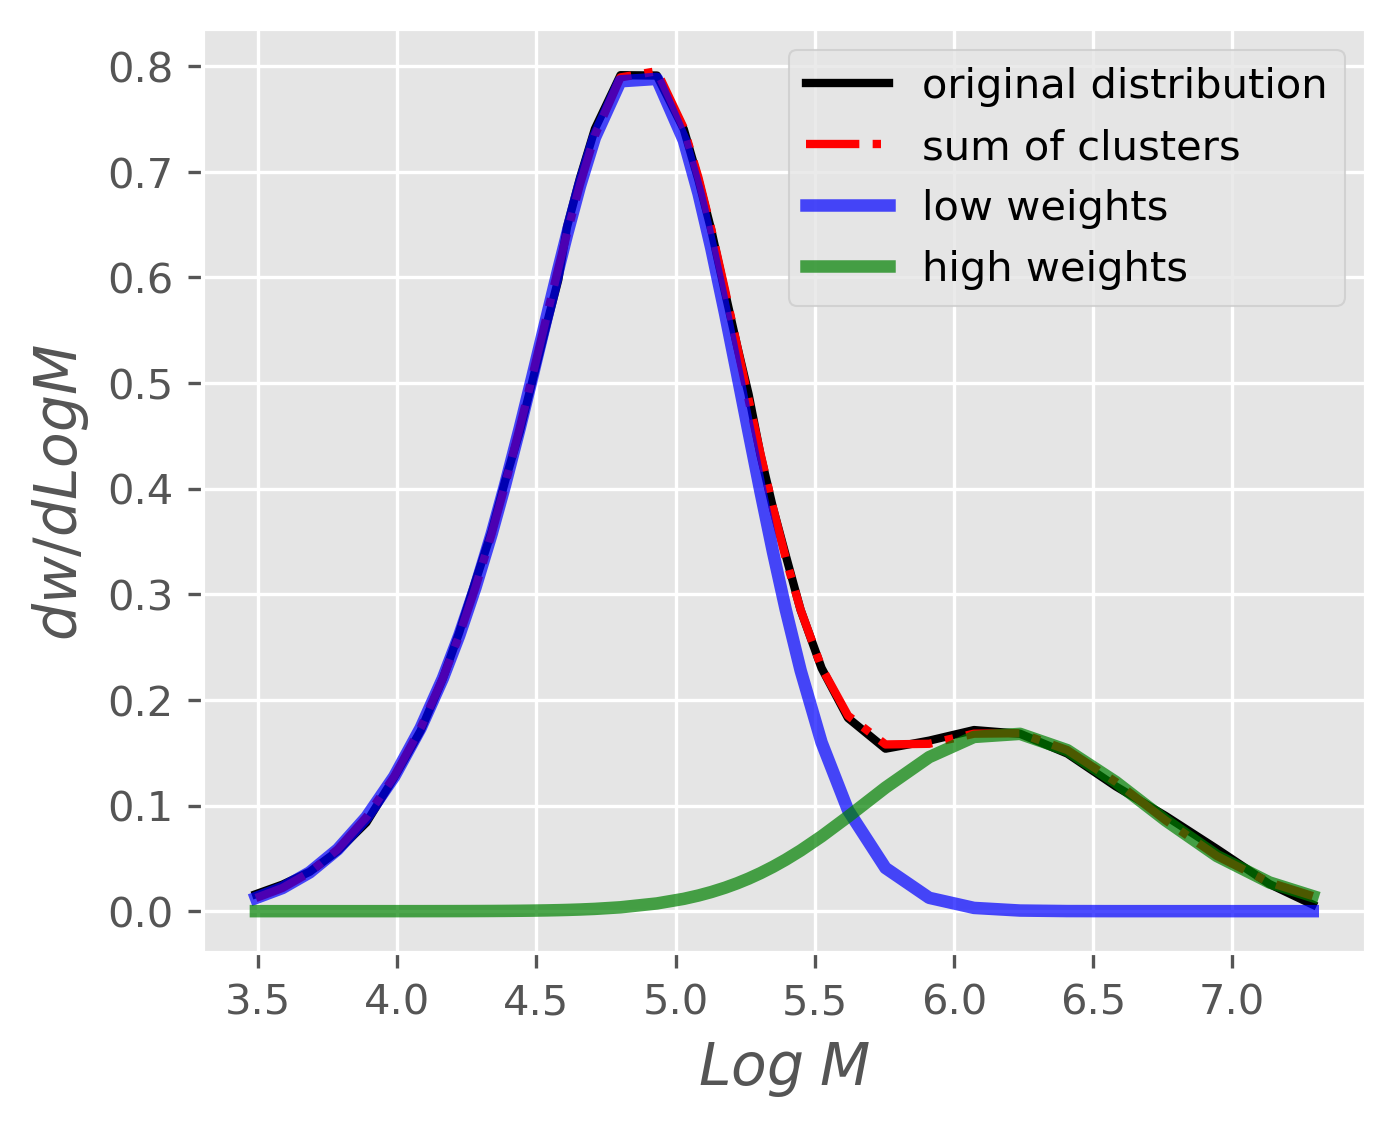
\includegraphics[scale=1]{figures/deconvoluted}
	\caption{Peak deconvolution using ML}
	\end{center}
\end{figure}



\begin{abstract}
This project makes use of machine learning to perform peak deconvolution. A classification algorithm is used to segment polymer chains distribution into subpopulations corresponding to their production site.
\end{abstract}


\section*{Motivation}
The motivation for this project is to overcome the challenge a user faces during peak deconvolution, that is, the need to provide the expected peak locations for deconvolution to be done.

\section*{Key insight}
By using machine learning to identify clusters in a distribution, peak deconvolution can easily be performed. This method most often leads to more reliable results.

\section*{Introduction}
In polymer science the mechanical properties of a plastic material greatly depends on the characteristics of the two major subpopulations. These populations can be tweaked to produce materials of desirable properties, hence it is sometime required to perform peak deconvolution to fully account for the role played by each population. This has traditionally been achieved by making use commercial softwares. In this project we will using the expectation-maximization algorithm to identify the clusters and subsequently perform deconvolution.
\section*{Results and discussion}
\subsection*{Choice of model}
There are several models which could be used for classification such as K-Nearest Neighbors. Our choice of the Gaussian mixture model in this project was because, not only can it be used for classification purposes but also it can be used as a kernel estimator (see file on data preparation).
\subsection*{Optimizing the number of clusters}
The number of clusters required to fully represent the distribution and their characteristics are unknown from the start. To obtain that, we looped over $n$ of possible clusters
\begin{itemize}
	\item perform classification
	\item use the cluster parameters to generate a gaussian distribution (ie the chains produce at a site follows a gaussian distribution)
	\item calculate the difference between the area under the curve of the original distribution and the sum of the distribution from the clusters [plotted in figure 2]
\end{itemize} 
\begin{figure}[!htb]
	\begin{center}	
	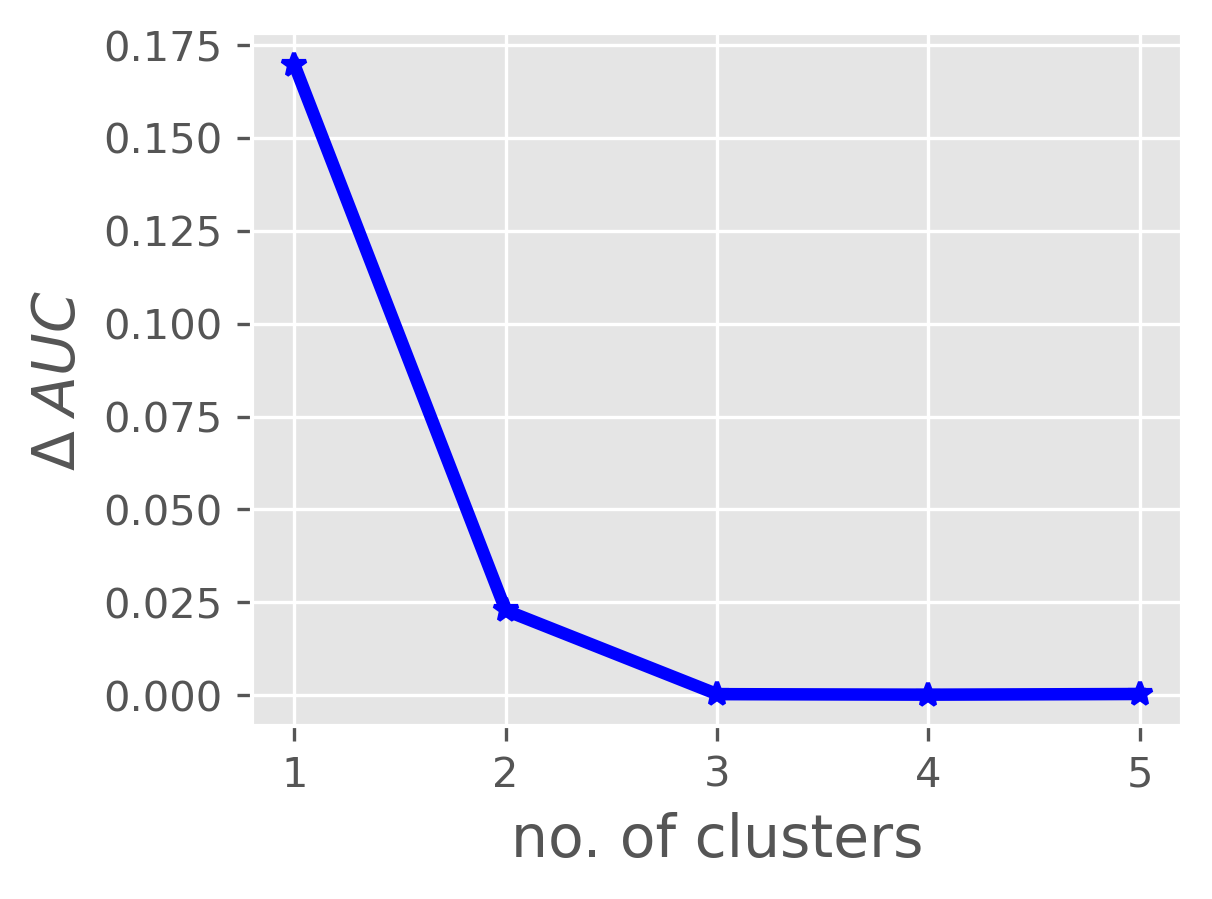
\includegraphics[scale=1]{figures/error_curve}
	\caption{Calculation of error}
	\label{fig:error}
	\end{center}
\end{figure}
From Fig.\ref{fig:error}, the error seems to be minimal when using 3 cluster, beyond which no further usefull information is obtained. 

\begin{figure}[!htb]
	\begin{center}
	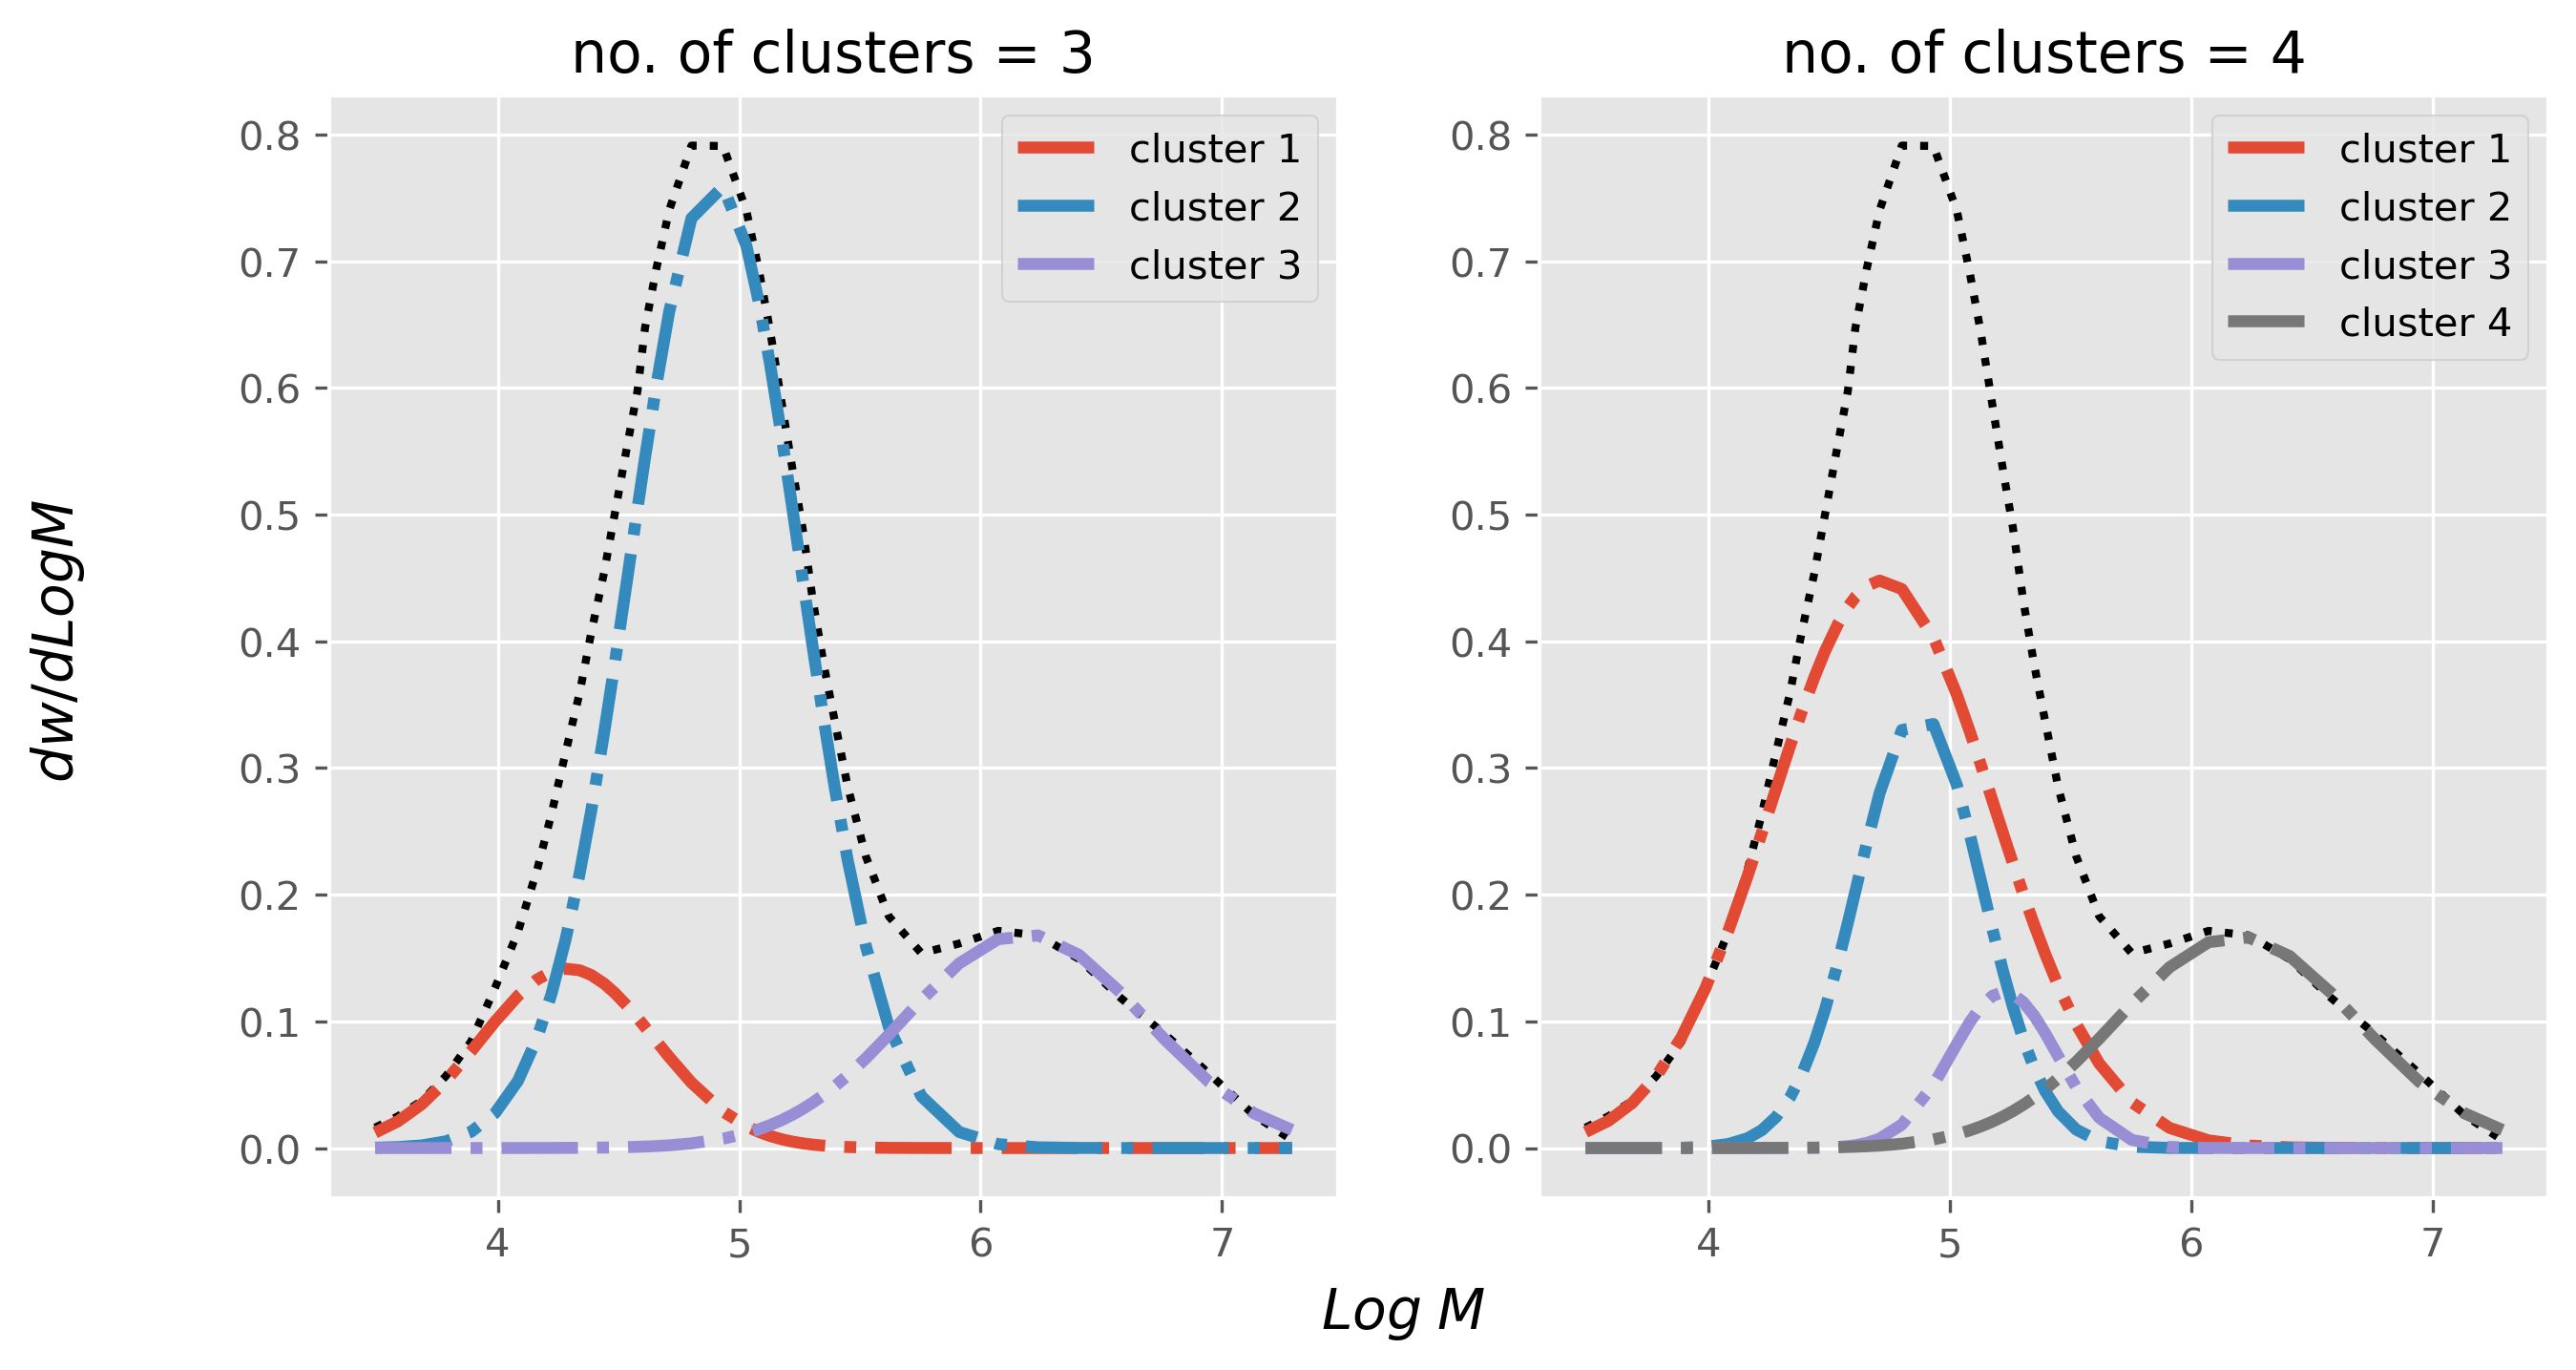
\includegraphics[width=\textwidth]{figures/comparison_nclusters}
	\caption{comparing output of 3 and 4 clusters}
	\label{fig:comparison}
	\end{center}
\end{figure}
 This can be observed from Fig.\ref{fig:comparison}, where the curve on the right has cluster 2 and 3 are all embedded in cluster 1



\end{document}